\documentclass[conference]{IEEEtran}
\IEEEoverridecommandlockouts
% The preceding line is only needed to identify funding in the first footnote. If that is unneeded, please comment it out.
\usepackage{cite}
\usepackage{amsmath,amssymb,amsfonts}
\usepackage{algorithmic}
\usepackage{graphicx}
\usepackage[hidelinks]{hyperref}
\usepackage{textcomp}
\usepackage{xcolor}
\def\BibTeX{{\rm B\kern-.05em{\sc i\kern-.025em b}\kern-.08em
    T\kern-.1667em\lower.7ex\hbox{E}\kern-.125emX}}
\begin{document}

\title{Analyzing Object Storage Backends for JULEA}
% \\
% {\footnotesize \textsuperscript{*}https://dblp.org/rec/conf/supercomputer/Kuhn17.html?view=bibtex}
% }

\author{\IEEEauthorblockN{Kseniya Shastakova}
\IEEEauthorblockA{\textit{Data-Intensive Applications and Systems Laboratory} \\
\textit{Swiss Federal Institute of Technology Lausanne}\\
Lausanne, Switzerland \\
shestakova.ko@phystech.edu}
\and
\IEEEauthorblockN{Kira Duwe}
\IEEEauthorblockA{\textit{Data-Intensive Applications and Systems Laboratory} \\
\textit{Swiss Federal Institute of Technology Lausanne}\\
Lausanne, Switzerland \\
kira.duwe@epfl.ch}
\and
\IEEEauthorblockN{Anastasia Ailamaki}
\IEEEauthorblockA{\textit{Data-Intensive Applications and Systems Laboratory} \\
\textit{Swiss Federal Institute of Technology Lausanne}\\
Lausanne, Switzerland \\
anastasia.ailamaki@epfl.ch}
}

\maketitle

\begin{abstract}
Modern life involves processing unimaginable amounts of data. For example, applications connected with weather forecasting and artificial intelligence are very intensive in terms of data usage. However, it is not enough to process data at the moment. To make data management more effective, one should be able to refer to the results of previous work. This is achieved with the help of storage systems. One particular case of storage is object storage, which provides a simple yet efficient interface for manipulating data. In this work, we used several object storage clients to implement the object storage backend for JULEA, a flexible framework for prototyping new approaches in storage management and compared them in terms of efficiency and usability. The final recommendation suggested by the work is to use the AWS C++ SDK for the implementation of the JULEA object storage backend.
\end{abstract}



\section{Introduction}
In recent years, the number of applications used in daily routines has increased. Along with that, applications have become more data-intensive. For example, ChatGPT was initially trained on 570 GB of data.
Currently, the archive of meteorological data of the German Climate Computing Center (DKRZ) has a capacity of 300 PB~\cite{NODBLP:dkrz-archive-size}.  For efficient management of such amounts of data, a well-elaborated storage system is required. 
In high-performance computing (HPC), such systems are typically distributed and parallel file systems that run on a supercomputer~\cite{DBLP:journals/superfri/Luttgau0DABK018}.
However, systems like Lustre~\cite{DBLP:conf/sc/TaoDBN12} have a high complexity and are run in the kernel, which comes with drawbacks for teaching and smaller research projects, especially in terms of development and deployment without root privileges. This work uses JULEA~\cite{DBLP:conf/supercomputer/Kuhn17} as a flexible framework for prototyping new approaches in storage management.
The simplicity of object storage makes it a good solution for a wide range of data management problems, including teaching and prototyping new ideas. However, clients for object storage differ in terms of performance, compatibility with servers, and the range of features provided. This work compares OpenIO~\cite{NODBLP:openio}, AWS~\cite{NODLBP:aws} and MinIO~\cite{NODLBP:minio} object storage clients in terms of efficiency and usability and provides a final recommendation for further JULEA object storage backend development.

\section{Background}

This section covers fundamental aspects of the different object store solutions that are evaluated in this paper as well as the general JULEA architecture.
HPC systems and cloud servers tend to choose object storage for the encapsulation of complex data management. Object storage has two main entities: an object and a bucket. Supporting arbitrary structure and metadata, a bucket is a flexible analogue of the file in a traditional file system. Buckets are containers for objects with a flat hierarchy. Thus, object storage is a simple solution for data processing. However, it is impossible for storage to exist separately from applications. In this work, the application layer is presented by JULEA~\cite{DBLP:conf/supercomputer/Kuhn17}. JULEA is a flexible framework that was originally designed for teaching purposes and thus can be easily adopted for prototyping new storage solutions. Another important feature of JULEA is that it is completely user-space, which makes it easy to test and debug backends inside the framework. Analyzing the process of application-storage communication, presented in Figure~\ref{fig:app-storage-communication}, leads to the conclusion that client-server communication is a bottleneck for applications.

\begin{figure}
    \centering
    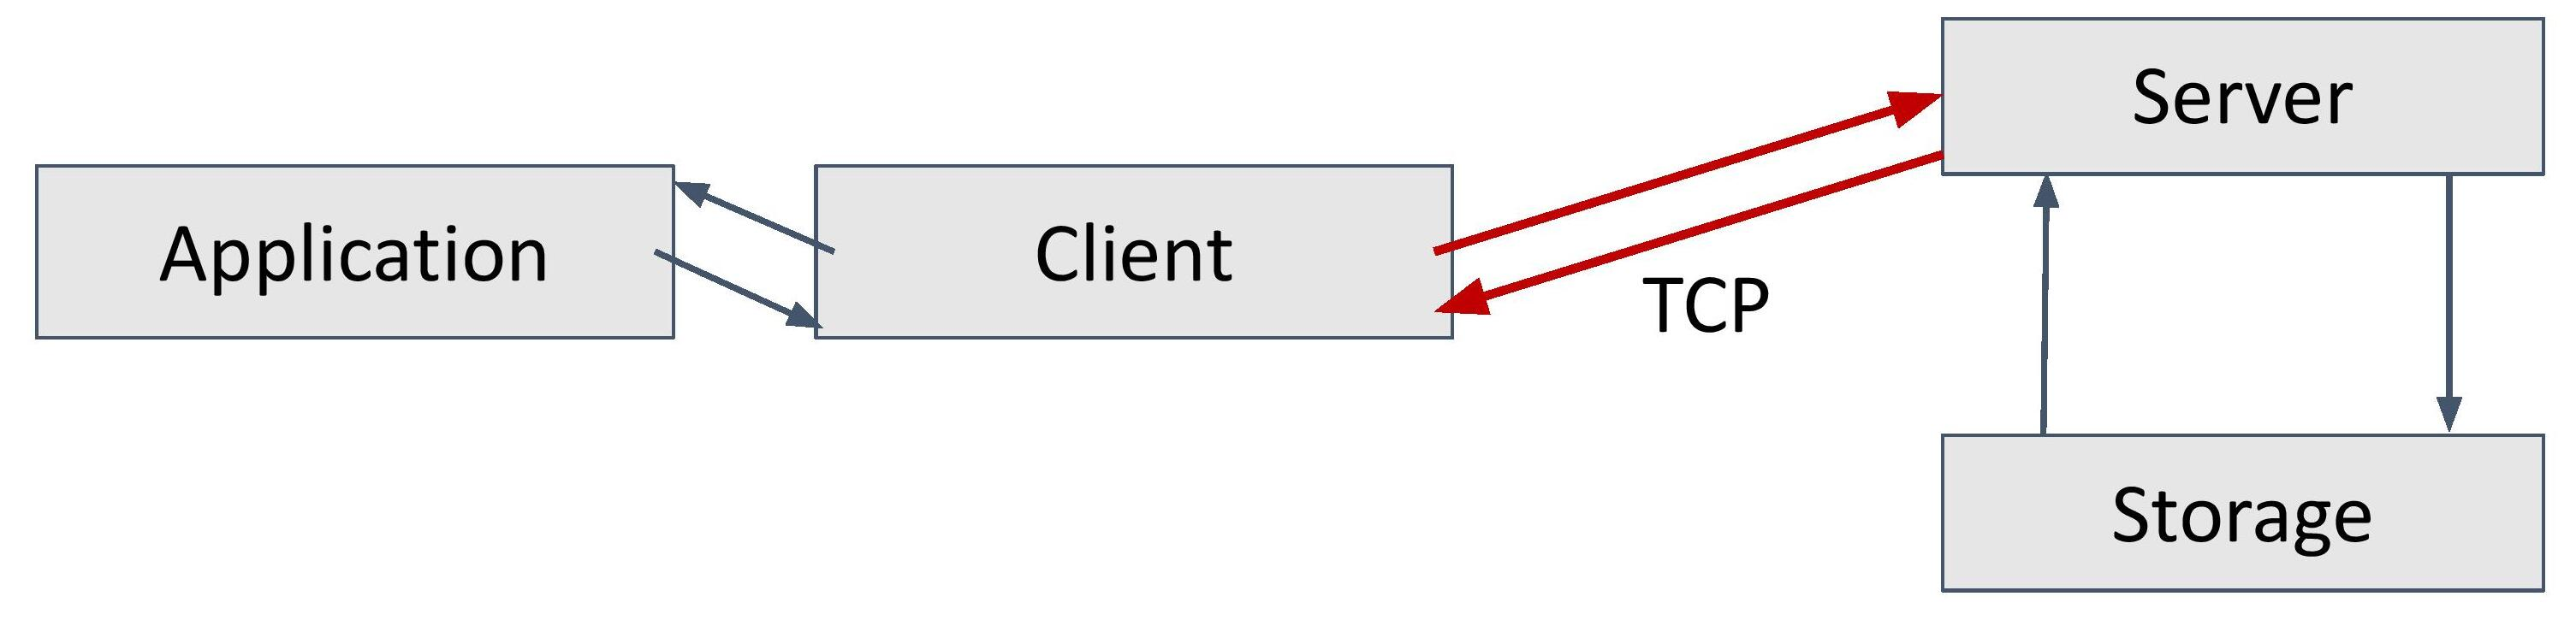
\includegraphics[width=0.85\linewidth]{keseniya-internship-presentation.pptx-4-page-001 (1).jpg}
    \caption{Application-Storage communication}
    \label{fig:app-storage-communication}
\end{figure}

\subsection{OpenIO C SDK}
In an ideal world, clients should not matter, but in reality, clients differ in terms of compatibility with servers, supported features and efficiency. Thus, the overall performance of the application is not defined only by the server. For choosing the most efficient backend solution for JULEA, we considered the OpenIO C SDK, MinIO C++ SDK, and AWS C++ SDK. OpenIO turned out not to be a working solution. On the other hand, we were able to develop JULEA backends using MinIO and AWS C++ SDK. In order to find out which client is more efficient, evaluations were carried out. Finally, we compared MinIO and AWS C++ SDKs in terms of having understandable documentation, a wide developer community, supported features and simplicity of setting up. 
OpenIO C SDK is an open-source client for accessing the OpenIO object storage server. Originally, it was chosen for JULEA backend implementation because JULEA is written completely in C. Consequently, dealing with a backend implemented in C was significantly easier than dealing with one in any other programming language. However, while working with the OpenIO C SDK, multiple difficulties occur. First, the only Linux distribution for which OpenIO C SDK library building is supported is Ubuntu 18.04. Thus, for building the library, one needs to set up a Docker container running Ubuntu 18.04. However, it is impossible to run applications using methods from OpenIO on Ubuntu 18.04. For accessing the server, OpenIO developers provide a Docker container with CentOS 7 as an operational system. This Docker container runs the OpenIO server. The OpenIO user guide suggests changing the configuration file on the local machine to that of CentOS 7 for accessing the server remotely, but this approach did not work in my case. Thus, the only way of running applications accessing OpenIO server with OpenIO C SDK was by writing code and compiling it inside the Ubuntu 18.04 docker container, using the host machine to transfer executables from it to the CentOS 7 docker container, and running code inside the last mentioned container. However, this approach is inapplicable for running the OpenIO JULEA backend because, for doing that, a single machine able to run both JULEA and OpenIO is required, but CentOS 7 cannot be used for running JULEA. In conclusion, issues arising while working with OpenIO make it inapplicable for writing a JULEA backend.

\subsection{MinIO and AWS C++ SDK}
For further research, the MinIO and AWS C++ SDKs were chosen. As it was mentioned above, JULEA is written completely in C. Thus, it is necessary to write a wrapper or a translation layer for C++ SDK before it can be used in a JULEA backend.
MinIO C++ SDK is an AWS S3-compatible object storage API that can also be run on MinIO servers. Referring to GitHub issues and developer comments suggests that the MinIO C++ SDK potentially has thread-safety issues. On the other hand, AWS C++ SDK is the standard API for the AWS S3 object storage server. However, it can work not only with AWS servers but also with MinIO servers. The library of the AWS C++ SDK is well-elaborated and contains a lot of useful features that can be later used for optimizing the backend. At first glance, the AWS and MinIO C++ SDKs look similar: both are written in C++, both were originally built with CMake, and both can be run on MinIO servers. However, in our research, the MinIO C++ SDK was run on the MinIO playground, while the MinIO localhost server was used for running the AWS client. It can be explained this way. Both clients use the IP address of the server to access it. When providing the IP address of the MinIO playground server to the AWS client, a connection error occurs. The same situation happens when providing the IP address of localhost to a MinIO client. Thus, the configuration mentioned earlier is the only one that works. MinIO and AWS C++ SDKs also differ in terms of setting them up manually. MinIO C++ SDK library has multiple dependencies, while AWS requires only CURL, which is a basic tool supported by most systems. Thus, the two considered clients differ in terms of compatibility with servers, supported features and setting up manually. However, this information says nothing about the performance of the clients. Consequently, evaluations are required for a more objective comparison of the AWS and MinIO C++ SDKs.

\section{Evaluation}
All the evaluations were run on ASUS TUF Gaming F15 FX506LI\_FX as a host machine, with an operational system of Ubuntu 21.10 x86\_64 on kernel 5.13.0-52-generic, a CPU of the Intel i5-10300H (4,500 GHz frequency), 56 GB of SSD memory available, and 8 GB of RAM.

\subsection{Overall Comparison}
For a brief comparison of the AWS and MinIO C++ SDKs, nine test suites were used. Each of the suites included multiple repetitions of one of the following functions in different combinations: open, close, create, delete, read, and write. For the AWS C++ SDK, each test suite affected 500 objects and was repeated 38 times, while for the MinIO C++ SDK, 10 objects were affected per test, and each test suite was executed 18 times. The result of the tests is presented in Figure~\ref{fig:overall-comparison}. 
\begin{figure}
    \centering
    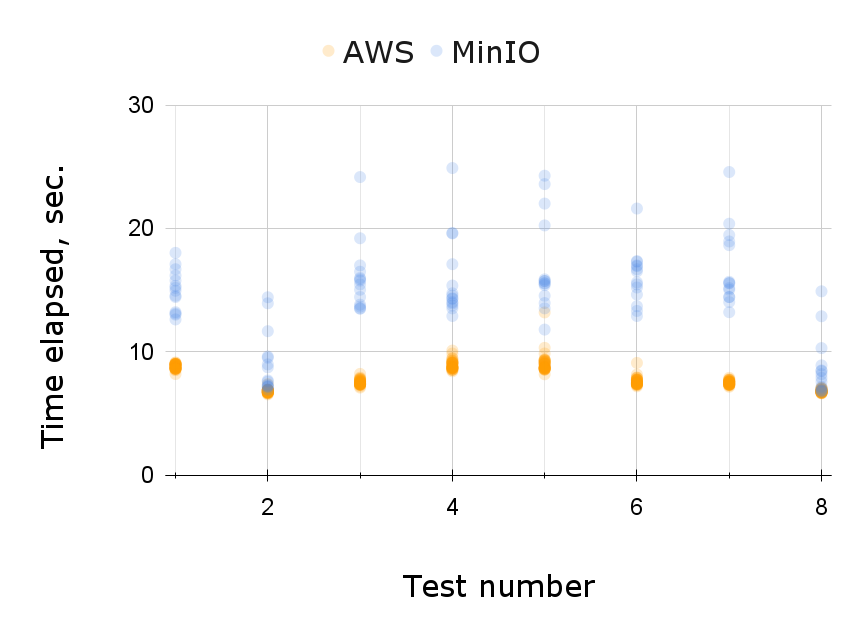
\includegraphics[width=0.9\linewidth]{overall_comparison.png}
    \caption{Overall comparison}
    \label{fig:overall-comparison}
\end{figure}
It illustrates that despite the fact that the number of objects retrieved per test for AWS is 50 times bigger than for MinIO, the average time elapsed per test for AWS is smaller than for MinIO. At the same time, the plot shows that the difference between the largest time elapsed and the smallest one is significantly bigger for MinIO than for AWS. Thus, MinIO performance is slower and less stable than that of AWS. The obtained result suggests giving up the idea of using the MinIO C++ SDK for JULEA backend development. However, this result is not sufficient to claim that the AWS C++ SDK is a proper solution for the JULEA object storage backend implementation. To verify if it is, evaluations for particular use cases were carried out.

\subsection{Read And Write Performance of AWS C++ SDK Based on the Block Size}
For verifying the relation between number of bytes read and time elapsed, tests with read sizes of 512, 1024, 2048, 4096, 8192, 12288, 16384, and 32768 bytes were run. The results of these tests are shown in Figure~\ref{fig:read-block-size}.
\begin{figure}
    \centering
    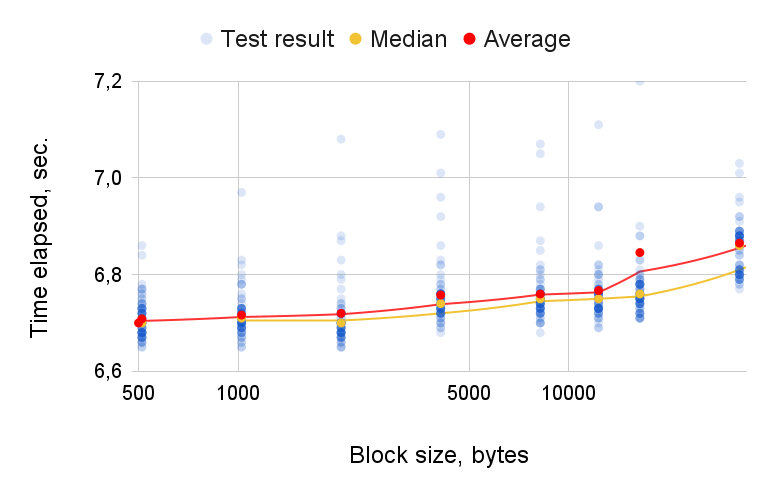
\includegraphics[width=0.9\linewidth]{read_bs.png}
    \caption{Read performance based on block size}
    \label{fig:read-block-size}
\end{figure}
The x-axis is presented on a logarithmic scale. In spite of the fact that the size of blocks grows exponentially, the time elapsed does not increase exponentially. For block sizes from 512 to 16384, the relation looks almost linear, while for 32768, a jump is observed for both the average and median. Thus, there is no clear relation between the block size and time elapsed. The same block sizes were used for determining the relationship between write performance and block size. The results of the evaluation are presented in the graph.
Figure~\ref{fig:write-block-size} shows that the trend for the median for the write operation is similar to the median trend for the read operation, while the trend for the average looks more chaotic. It is so because the average is badly affected by outliers. This observation suggests that write performance is less stable than read performance.

\begin{figure}
    \centering
    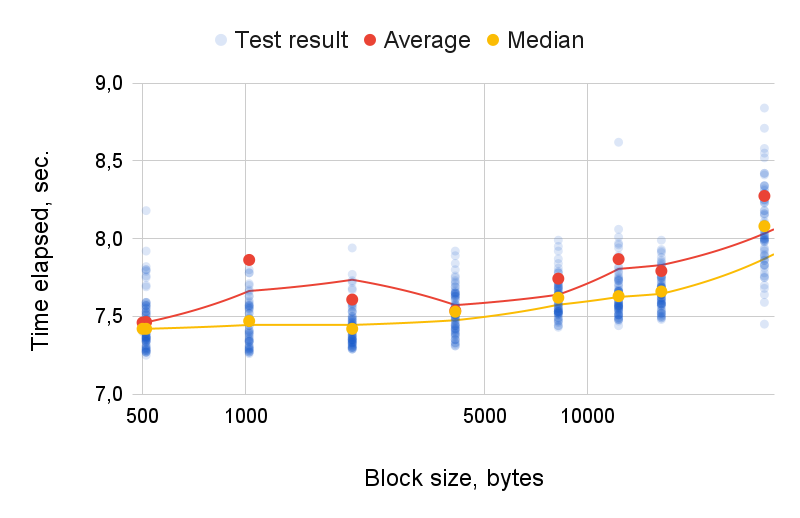
\includegraphics[width=0.9\linewidth]{write_bs_1.png}
    \caption{Write performance based on block size}
    \label{fig:write-block-size}
\end{figure}

\subsection{Read and Write Performance of AWS C++ SDK Based on Number of Objects Affected}
For determining the relation between the number of objects retrieved per test and time elapsed, tests with a reading size of 200, 400, 600, 800, and 1000 objects were run. The results of these tests are presented in Figure~\ref{fig:read-objects-number}. 
\begin{figure}
    \centering
    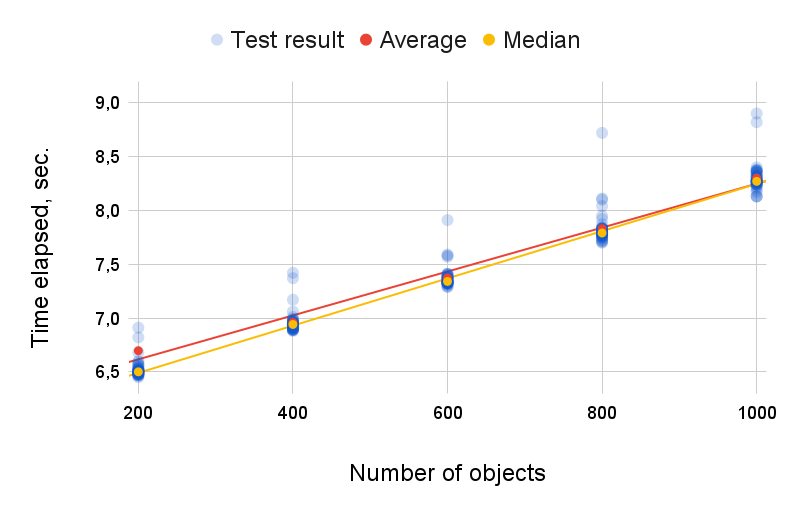
\includegraphics[width=0.9\linewidth]{read_nod.png}
    \caption{Read performance based on number of objects}
    \label{fig:read-objects-number}
\end{figure}
The plot illustrates that there is a clear linear relationship between the average or median time elapsed and the number of objects affected per test. Tests with the mentioned numbers of objects were also run for the write operation, with results provided in Figure~\ref{fig:write-objects-number}.
\begin{figure}
    \centering
    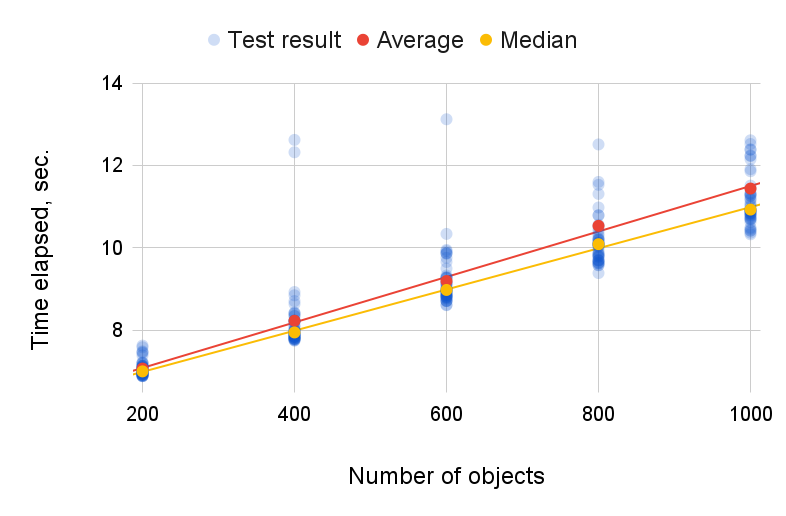
\includegraphics[width=0.9\linewidth]{write_nod.png}
    \caption{Write performance based on number of objects}
    \label{fig:write-objects-number}
\end{figure}
For write, a linear relation is also observed, though the difference between average and median is bigger than that of read. It can be explained by outliers. 

At this point, it is necessary to mention that the performance of the AWS write operation is less stable than that of the read operation. However, it is not a big problem because in a common use case of object storage, the content is written once and read multiple times, so read performance is more important than write performance. 

\section{Conclusion}
The results provided above show that OpenIO is inapplicable for a new JULEA backend because of setup and execution issues. On the other hand, both MinIO and AWS provide interfaces necessary for the backend implementation. However, the AWS C++ SDK has proven to be a better solution for the following reasons. Firstly, the AWS client on the localhost MinIO server performs faster and is more stable than the MinIO client on the MinIO playground server. Secondly, AWS has a more well-elaborated library with multiple useful features that can be used later for optimizing the backend. Along with that, AWS is better documented, and the community of AWS is bigger than that of MinIO, which makes it easier to deal with difficulties that occur while using this library. Thus, the final recommendation is to use AWS for a new JULEA backend. 


% \begin{thebibliography}{00}
% \bibitem{b1} Michael Kuhn. 2017. JULEA: A Flexible Storage Framework for HPC. 
% \bibitem{b2} Dinesh Kalla, Nathan Smith. March 2023. Study and Analysis of Chat GPT and its Impact on Different Fields of Study. In International Journal of Innovative Science and Research Technology ISSN No:-2456-2165, Volume 8, Issue 3, March – 2023.
% \bibitem{b3} KOREA METEOROLOGICAL ADMINISTRATION Annual Report 2017. Web. https://www.kma.go.kr/download\_01/Annual\_Report\_2017.pdf

% \end{thebibliography}

\bibliographystyle{plain}
\bibliography{paper}

\end{document}
